%
% Curriculum vitae for Michael L. Miller (v1, 11-Dec-2016)
%
% Based on Joseph D. Monaco (jdmonaco-cv.tex) downloaded from https://github.com/jdmonaco on 11-December-2016
% For the initial template h/t Matthew M. Boedicker <mboedick@mboedick.org> http://mboedick.org
% $Id: resume.tex,v 1.7 2004/02/02 14:21:06 mboedick Exp $
%

\documentclass[10pt, singleside]{article}
\usepackage{fullpage}
\usepackage{palatino}
\usepackage[hidelinks]{hyperref}
\usepackage{multirow}
\usepackage{tabu}
\usepackage{graphicx}
\usepackage{fancyhdr}
\textheight=9.5in
\raggedbottom
\raggedright
\usepackage{geometry}
 \geometry{
 	left=1.25cm,
	right=1.25cm,
 	top=2cm,
	bottom=1cm,
 }
\pagestyle{fancy}
\setlength{\tabcolsep}{0in}
\addtolength{\voffset}{-.4in}
%\addtolength{\textheight}{.9in}
%\addtolength{\hoffset}{-.25in}
%\addtolength{\textwidth}{.2in}
\fancyhf{}
\renewcommand{\headrulewidth}{0pt}
\renewcommand{\footrulewidth}{0.5pt}
%\renewcommand{\footskip}{0}
%\fancyfoot[CE,CO]{\leftmark}
\fancyfoot[L]{\em{Miller, ML}}
\fancyfoot[C]{\thepage}
\fancyfoot[R]{Last updated on 11-Dec-2016}


\begin{document}

\begin{tabular*}{7.5in}{c@{\extracolsep{\fill}}rl}
\hline\\[0.01in]
%\multirow{5}{*}{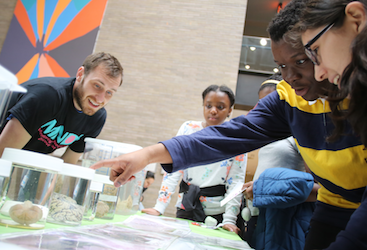
\includegraphics[scale=0.15]{/Users/Mike/Desktop/Untitled.png}} 
\textsc{\textbf{\Large Michael Lawrence Miller, Ph.D.}}	& \textsc{Phone}	& \texttt{+1-516-244-0672} \\
\multirow{2}{*}{\large }                                & \textsc{E-mail}      & \href{mailto:michael.miller@icahn.mssm.edu}{\texttt{michael.miller@icahn.mssm.edu}} \\
\href{http://icahn.mssm.edu}{\small Icahn School of Medicine at Mount Sinai}    & \textsc{Web}        & \href{http://millem14.u.hpc.mssm.edu/}{\texttt{millem14.u.hpc.mssm.edu}} \\
\href{https://www.google.com/maps/place/Icahn+School+of+Medicine+at+Mount+Sinai/@40.79051,-73.9512909,17z/data=!4m5!3m4!1s0x0:0x2593c320cab0ef41!8m2!3d40.7898697!4d-73.9533614}{\small One Gustave L. Levy Place}              & \textsc{Google Scholar}      & \href{https://scholar.google.com/citations?user=7EVp2IkAAAAJ}{\texttt{7EVp2IkAAAAJ}} \\
\href{https://www.google.com/maps/place/Icahn+School+of+Medicine+at+Mount+Sinai/@40.79051,-73.9512909,17z/data=!4m5!3m4!1s0x0:0x2593c320cab0ef41!8m2!3d40.7898697!4d-73.9533614}{\small New York, NY, 10029, USA}                      & \textsc{Doximity}   & \href{http://www.doximity.com/profile/6396828}{\texttt{6396828}} \\[0.1in]
\hline
\end{tabular*}

\vspace{0.15in} {\large \textbf{Education}}

\begin{itemize}
  \item 
  \begin{tabular*}{7.15in}{l@{\extracolsep{\fill}}r}
    \textbf{Icahn School of Medicine at Mount Sinai} & New York, NY \\
    Medical Scientist Training Program (MSTP) & 2010--present \\
    Ph.D. in Neuroscience (2016), M.D. (expected, May 2018) \\
    Dissertation Title: \textit{Genetic and epigenetic risk factors of opiate abuse}
  \end{tabular*}
  \item 
  \begin{tabular*}{7.15in}{l@{\extracolsep{\fill}}r}
    \textbf{Binghamton University} & Binghamton, NY \\
    B.S. in Integrative Neuroscience, B.S. in Biochemistry, & 2006--10\\
    Dean's Certificate in evolutionary studies \\
    \textit{Summa cum laude} \\
  \end{tabular*}
\end{itemize}

{\large \textbf{Research Experience}}
\begin{itemize}
\item
  \begin{tabular*}{7.15in}{l@{\extracolsep{\fill}}r}
    \textbf{Icahn School of Medicine at Mount Sinai} & New York, NY\\
    Fishberg Department of Neuroscience, Friedman Brain Institute & 2012--present \\
    Graduate Student, MSTP \\
    Dissertation Advisor: Yasmin L. Hurd, Ph.D. \\
  \end{tabular*}
\item
  \begin{tabular*}{7.15in}{l@{\extracolsep{\fill}}r}
    \textbf{Brookhaven National Laboratories} & Upton, NY\\
    Department of Medicine & 2008--10 \\
    Summer Undergraduate Researcher \\
    Supervisor: Panayotis (Peter) K. Thanos, Ph.D. \\
  \end{tabular*}
\item
  \begin{tabular*}{7.15in}{l@{\extracolsep{\fill}}r}
    \textbf{Binghamton University} & Binghamton, NY\\
    Department of Biological Sciences & 2007--10 \\
    Undergraduate Researcher \\
    Honor's Thesis Advisor: Anne B. Clark, Ph.D. \\
  \end{tabular*}
\end{itemize}

{\large \textbf{Grants and Fellowships}}

\begin{itemize}
\item
	\begin{tabular*}{7.15in}{l@{\extracolsep{\fill}}r}
  		\textbf{Ruth L. Kirschstein National Research Service Award Fellow} &	2015--present	\\
		National Institute on Drug Abuse, National Institutes of Health &	\$171,370 \\
		Project title: \textit{Identifying distinct striatonigral and striatopallidal disturbances} \href{https://projectreporter.nih.gov/project_info_description.cfm?aid=9024346}{(F30-DA-038954)} \\
  	\end{tabular*}
\item
	\begin{tabular*}{7.15in}{l@{\extracolsep{\fill}}r}
  		\textbf{Barry M. Goldwater Scholar in Mathematics, Science and Engineering} &	2009--2010	\\
   		The Barry M. Goldwater Foundation &	\$7500 \\
  	\end{tabular*}
\end{itemize}

{\large \textbf{Publications}}

\begin{description}
\item Miller ML \& Hurd YL. (in press). Testing the gateway drug hypothesis. \textit{Neuropsychopharmacology}.
\item Egervari G, Jutras-Aswad D, Landry J, \textbf{Miller ML}, Anderson SA, Michaelides M, Jacobs MM, Peter C, Yiannoulos G, Liu X, \& Hurd YL. (2016). A functional 3'UTR polymorphism (rs2235749) of Prodynorphin alters microRNA-365 binding in ventral striatonigral neurons to influence novelty seeking and positive reward traits. \textit{Neuropsychopharmacology}, \textit{10}, 2512-2520. \href{http://dx.doi.org/10.1038/npp.2016.53}{doi:~10.1038/npp.2016.53}.
\item Thanos PK, Michaelides M, Subrize M, \textbf{Miller ML}, Bellezza R, Cooney RN, Leggio L, Wang G-J, Rogers AM, Volkow ND, \& Hajnal A. (2015). Roux-en-Y gastric bypass alters brain activity in regions that underlie reward and taste perception. \textit{PLoS One}, \textit{10}, e0125570. \href{http://dx.doi.org/10.1371/journal.pone.0125570}{doi:~10.1371/journal.pone.0125570}.
\item \textbf{Miller ML}, Chadwick B, Morris CV, Michaelides M, \& Hurd YL. (2015). Cannabinoid-Opioid Interactions. In P. Campolongo \& L. Fattore (Eds.) \textit{Cannabinoid Modulation of Emotion Memory and Motivation} (pp 393-407) New York NY: Springer New York. \href{http://dx.doi.org/10.1007/978-1-4939-2294-9_15}{doi:~10.1007/978-1-4939-2294-9\_15}.
\item Maze I, Chaudhury D, Dietz DM, von Schimmelmann M, Kennedy PJ, Lobo MK, Sillivan SE, \textbf{Miller ML}, Bagot RC, Sun H, Turecki G, Neve RL, Hurd YL, Shen L, Han M-H, Schaefer A, \& Nestler EJ. (2014). G9a influences neuronal subtype specification in striatum. \textit{Nature Neuroscience}, \textit{17}, 533-539. \href{http://dx.doi.org/10.1038/nn.3670}{doi:~10.1038/nn.3670}.
\item Szutorisz H, DiNieri JA, Sweet E, Egervári G, Michaelides M, Carter JM, Ren Y, \textbf{Miller ML}, Blitzer RD, \& Hurd YL. (2014). Parental THC exposure leads to compulsive heroin-seeking and altered striatal synaptic plasticity in the subsequent generation. \textit{Neuropsychopharmacology}, \textit{39}, 1315-1323. \href{http://dx.doi.org/10.1038/npp.2013.352}{doi:~10.1038/npp.2013.352}.
\item Chadwick B, \textbf{Miller ML}, \& Hurd YL. (2013). Cannabis use during adolescent development: susceptibility to psychiatric illness. \textit{Frontiers in Psychiatry}, \textit{4}, 129. \href{http://dx.doi.org/10.3389/fpsyt.2013.00129}{doi:~10.3389/fpsyt.2013.00129}.
\item Hurd YL, Michaelides M, \textbf{Miller ML}, \& Jutras-Aswad D. (2013). Trajectory of adolescent cannabis use on addiction vulnerability. \textit{Neuropharmacology}, \textit{76}, 416-424. \href{http://dx.doi.org/10.1016/j.neuropharm.2013.07.028}{doi:~j.neuropharm.2013.07.028}.
\item Michaelides M, \textbf{Miller ML}, Subrize M, Kim R, Robison L, Hurd YL, Wang G-J Volkow ND, \& Thanos PK. (2013). Limbic activation to novel versus familiar food cues predicts food preference and alcohol intake. \textit{Brain Research}, \textit{1512}, 37-44. \href{http://dx.doi.org/10.1016/j.brainres.2013.03.006}{doi:~10.1016/j.brainres.2013.03.006}.
\item \textbf{Miller ML}, Gallup AC, Vogel AR, Vicario SM, \& Clark AB. (2012). Evidence for contagious behaviors in budgerigars (\textit{Melopsittacus undulatus}): An observational study of yawning and stretching. \textit{Behavioural Processes}, \textit{89}, 264-270. \href{http://dx.doi.org/10.1016/j.beproc.2011.12.012}{doi:~10.1016/j.beproc.2011.12.012}.
\item \textbf{Miller ML}, Gallup AC, Vogel AR, \& Clark AB. (2012). Auditory disturbances promote temporal clustering of yawning and stretching in small groups of budgerigars (\textit{Melopsittacus undulatus}). \textit{Journal of Comparative Psychology}, \textit{126}, 324-328. \href{http://dx.doi.org/10.1037/a0026520}{doi:~10.1037/a0026520}.
\item \textbf{Miller ML}, Gallup AC, Vogel AR, \& Clark AB. (2010). Handling-stress initially inhibits but then potentiates yawning in budgerigars (\textit{Melopsittacus undulatus}). \textit{Animal Behaviour}, \textit{80}, 615-619. \href{http://dx.doi.org/10.1016/j.anbehav.2010.05.018}{doi:~10.1016/j.anbehav.2010.05.018}.
\item Gallup AC, \textbf{Miller ML}, \& Clark AB. (2010). The direction and range of ambient temperature change influences yawning in budgerigars (\textit{Melopsittacus undulatus}). \textit{Journal of comparative Psychology}, \textit{124}, 133-138. \href{http://dx.doi.org/10.1037/a0018006}{doi:~10.1037/a0018006}.
\item Gallup AC, \textbf{Miller ML}, \& Clark AB. (2009). Yawning and thermoregulation in budgerigars: Science as an incremental process. \textit{Animal Behaviour}, \textit{78}, e3-e5. \href{http://dx.doi.org/10.1016/j.anbehav.2009.09.017}{doi:~10.1016/j.anbehav.2009.09.017}.
\item Gallup AC, \textbf{Miller ML}, \& Clark AB. (2009). Yawning and thermoregulation in parakeets (\textit{Melopsittacus undulatus}). \textit{Animal Behaviour}, \textit{77}, 109-113. \href{http://dx.doi.org/10.1016/j.anbehav.2008.09.014}{doi:~10.1016/j.anbehav.2008.09.014}.
\end{itemize}
\end{description}

\vspace{0.055in} {\large \textbf{Mentorship/Teaching}}

\begin{itemize}
\item
	\begin{tabular*}{7.15in}{l@{\extracolsep{\fill}}r}
  	\textbf{Teaching Assistant for Principles of Neurobiology: Systems Neuroscience} \\
   	Winter 2013, Directed by Elizabeth Cropper, Ph.D \\
  	\end{tabular*}
\item
	\begin{tabular*}{7.15in}{l@{\extracolsep{\fill}}r}
  	\textbf{Teaching Assistant for Brain \& Behavior} \\
   	Fall 2012, Directed by Carrie Ernst, M.D. \\
  	\end{tabular*}
\item
	\begin{tabular*}{7.15in}{l@{\extracolsep{\fill}}r}
  	\textbf{Undergraduate Teaching Assistant for Cellular Neurobiology} \\
   	Fall 2008 and Fall 2009, Directed by Carol I. Miles, Ph.D. \\
  	\end{tabular*}
\item
	\begin{tabular*}{7.15in}{l@{\extracolsep{\fill}}r}
  	\textbf{Mentored summer undergraduate interns and Master's students} \\
   	Judelca Rodriguez (Summer 2013), Nieghel Downer (\href{https://binghamton.edu/harpur/perspective/student/niegheldowner.html}{Summer 2014}), \\
	Yonaida Valentine (Summer 2015) and Tanni Rahman (2015-2016), \\
	Directed by Yasmin L. Hurd, Ph.D. \\
  	\end{tabular*}
\end{itemize}

%{\large \textbf{Presentations}}

\vspace{0.055in} {\large \textbf{Awards}}

\begin{itemize}
\item President’s Award for Undergraduate Student Excellence (2010), \$1000 
\item State University of New York Chancellor’s Award (2010)
\item John L. Fuller Memorial Award (2010), \$100
\item University Undergraduate Research Award (2009), \$250
\item University Undergraduate Research Award (2008), \$169 
\item Edward Thorsen Memorial Scholarship (2008), \$400 
\item Freshman Chemistry Award (Fall 2006, Spring 2007), \$50 each
\item Graduate Student’s GRC Poster Award (2013)
\item Brain Awareness Week Travel Award (2009), \$750 + conference registration
\item Sigma Xi Undergraduate Research Poster Award (2008, 2009), \$100 each
\item Department of Energy’s Summer Undergraduate Lab Internship (Summer 2009), \$3200 stipend 
\item Plainview Diner Scholarship (2006), \$500
\end{document}
